\documentclass[conference, a4paper]{IEEEtran}
\IEEEoverridecommandlockouts
% The preceding line is only needed to identify funding in the first footnote. If that is unneeded, please comment it out.
\usepackage[T1]{fontenc}
\usepackage{cite}
\usepackage{amsmath,amssymb,amsfonts}
\usepackage{algorithmic}
\usepackage{graphicx}
\usepackage{textcomp}
\usepackage{xcolor}
\usepackage{hyperref}
\usepackage[capitalise]{cleveref}
% \usepackage{natbib}
%max package
\usepackage[colorinlistoftodos]{todonotes}
% Bibliography


\def\BibTeX{{\rm B\kern-.05em{\sc i\kern-.025em b}\kern-.08em
    T\kern-.1667em\lower.7ex\hbox{E}\kern-.125emX}}
    
\begin{document}

\title{Towards the open source electricity network modelling of the African continent\
%\thanks{Include funding agency}
}
% ORDER OF AUTHORS TO BE FINALISED LATER - THIS IS JUST TO SEE HOW MUCH SPACE IT TAKES :)
\author{\IEEEauthorblockN{Desen Kirli}
\IEEEauthorblockA{\textit{Institute for Energy Systems} \\
\textit{University of Edinburgh}\\
Edinburgh, Scotland, United Kingdom \\
\href{mailto:desen.kirli@ed.ac.uk}{desen.kirli@ed.ac.uk} \\
\url{https://orcid.org/0000-0001-7596-0944}}
\and
\IEEEauthorblockN{Johannes Hampp}
\IEEEauthorblockA{\textit{Center for International Development} \\
\textit{and Environmental Research} \\
\textit{Justus-Liebig-University Giessen}\\
Giessen, Germany \\
\href{mailto:johannes.hampp@zeu.uni-giessen.de}{johannes.hampp@zeu.uni-giessen.de}\\
\url{https://orcid.org/0000-0002-1776-116X}}
\and
\IEEEauthorblockN{Koen van Greevenbroek}
\IEEEauthorblockA{\textit{Department of Computer Science} \\
\textit{UiT The Arctic University of Norway}\\
Tromsø, Norway \\
\href{mailto:koen.v.greevenbroek@uit.no}{koen.v.greevenbroek@uit.no} \\
\url{https://orcid.org/0000-0002-6105-2846}}
\and
\IEEEauthorblockN{Rebecca Grant}
\IEEEauthorblockA{\textit{Institute} \\
\textit{University of Edinburgh}\\
Edinburgh, Scotland, United Kingdom \\
\href{mailto:xxxx@ed.ac.uk}{xxxx@ed.ac.uk} \\
\url{https://orcid.org/}}
\and
\IEEEauthorblockN{Matin Mahmood}
\IEEEauthorblockA{\textit{School of Informatics} \\
\textit{University of Edinburgh}\\
Edinburgh, Scotland, United Kingdom \\
\href{mailto:M.Mahmood-3@sms.ed.ac.uk}{m.mahmood-3@sms.ed.ac.uk} \\
\url{https://orcid.org/}}
\and
\IEEEauthorblockN{Maximilian Parzen}
\IEEEauthorblockA{\textit{Institute for Energy Systems} \\
\textit{University of Edinburgh}\\
Edinburgh, Scotland, United Kingdom \\
\href{mailto:max.parzen@ed.ac.uk}{max.parzen@ed.ac.uk} \\
\url{https://orcid.org/0000-0002-4390-0063}}
\and
\IEEEauthorblockN{Aristides Kiprakis}
\IEEEauthorblockA{\textit{Institute for Energy Systems} \\
\textit{University of Edinburgh}\\
Edinburgh, Scotland, United Kingdom \\
\href{mailto:kiprakis@ed.ac.uk}{kiprakis@ed.ac.uk} \\
\url{https://orcid.org/0000-0001-7596-0944}}
}

\maketitle

\begin{abstract} %250 words
Electricity network modelling and grid simulations form the key for integrating newer and cleaner technologies such as renewable energy generators and electrical cars. This paper reviews the existing modelling packages and highlights the gap in the open source (OS) modelling of the African electricity network.
Using PyPSA (i.e. an OS Power System Analysis package), the paper outlines the pathway to a fully OS module and data to increase the transparency in the African network modelling.
Simulation of smart grid technologies will reveal the strong and weak parts of the grid which would accelerate their adoption in Africa and help with the strategic planning for upgrades and policy-making.
\end{abstract}

\begin{IEEEkeywords} % at least three, put in alphebetical order
Africa, open access, open source software, electricity access, geospatial modelling, network modelling, transmission system, electricity grid
\end{IEEEkeywords}

% \section*{Paper Guidelines from AFRICON2021}

% \begin{itemize}
% \item Papers should be written in English with a maximum paper length of \textcolor{red}{six (6) printed pages} (two-column format, 10-point font) using the supplied paper template including figures without incurring any page charges. 
% \item DEADLINE: \textcolor{red}{30/04/2021}
% \item all existing AFRICON proceedings live here since '92 \href{https://ieeexplore.ieee.org/xpl/conhome/1000025/all-proceedings}{\textbf{here}}
% \end{itemize}
 

\section{Introduction}
% \todo[inline]{Koen: personally, I would replace ``OS'' by ``open source'' everywhere. It doesn't save enough space to be worth the mental overhead of this abbreviation.}
The open source (OS) models and open-modelling initiatives in Europe bridge the gap between policymaking and long-term planning performed by researchers. For developing countries including but not limited to the ones located in the African continent, it is essential to simulate long-term energy generation and consumption scenarios as economic viability, risk and return on investments are key for investments in electrification and integration of renewable energy sources (RES).

Even though there are existing OS models and modelling tools in literature, there is a gap in evaluating the existing work that focuses specifically on Africa which is rich in many different kinds of RES such as solar and wind.
Here, we both provide a review of the most relevant work and also propose a roadmap to OS energy systems modelling in Africa.

The main contributions of this paper are outlines below:
\begin{itemize}
    \item A review of the existing OS energy systems models of Africa and categorisation of the existing work into academic and non-academic initiatives.
    \item A presentation of the proposed roadmap for our modelling initiative which has a focus on integration of RES and smart grid technologies such as batteries and electric vehicles.
\end{itemize}


\section{Review of the Existing Work, Initiatives and Motivation}
In this section, the motivation for OS modelling in Africa and drivers are outlined.
% such as rapid urbanisation, increasing population and development plans such as interconnection projects between African countries 
%%% WILL ADD REFERENCES HERE
Following this, we summarise the most relevant non-academic projects that promote OS energy modelling in the African continent. In the second subsection, we review the academic literature that feature existing OS models and simulation tools used for either the whole continent or a location in Africa. Lastly, we conclude this section by highlighting the gap that our proposed model plans to address.

\subsection{Motivation and non- academic existing projects for energy planning in Africa}
The main motivation behind most African energy models is to project the increasing rate of electrification linked to the rapid urbanisation, economic development and population growth in the African continent. 
% The case of Africa is interesting as... %cite some stats
% Start with electrification rate..increasing population, increasing electrification rate, GHG emissions, etc. using stats from IEA and EU Energy projections for African countries \href{https://op.europa.eu/en/publication-detail/-/publication/5bfffb22-fe1d-11e9-8c1f-01aa75ed71a1/language-en}{\textbf{here}}

In order to meet this predicted increase in electricity demand, respect limitations such as the green house gas (GHG) emissions and help implement the UN's Sustainable Development Goals (SDGs), the Paris Agreement and Africa´s Agenda 2063, different assets (e.g. wind turbines, batteries, etc.) and the African electricity transmission grid should be modelled. Additionally, other planned developments such as new transmission lines and similar should be taken into account in long-term energy modelling.
% It both teaches and promotes the use of open source modelling tools to help implement . 

% There are numerous initiatives to increase electrification and develop the resilience of the grid in Africa. One of the well-known methods for increasing resiliency is using introducing interconnection between countries such as the one between the UK and France. Despite the more complex modelling, simulation and computational costs, the advantages include higher system inertia and more stable frequency. 
\Cref{interconnector} (presented in the Conference on Power Transmission in Africa in 2019) shows the interconnection projects between various countries in Sub-Saharan Africa. This is an example of many initiatives that attempt to increase the resiliency of the African grid in order to prepare for the predicted increase in electrical demand.

\begin{figure}[t]
\centerline{\includegraphics[trim =  0.2cm 0cm 3cm 1.15cm, clip,width = 0.45\textwidth]{Figures/interconnector.jpg}}
\caption{Interconnector projects in Africa where red and blue denote feasibility and prefeasibility stages respectively. \footnote{1} }
\label{interconnector}
\end{figure}

% \todo[inline]{Question from Max: Do we need this Figure? Maybe we can position the Africa and EU map somewhere on top to inspire further reading? Eventhough the Figure 2 and 3 are mentioned later, there subscript is self-explanatory.
% Desen: I think it is necessary to include this - it explains the motivation. Can discuss it again once the first iteration is ready for a review.}
% \subsection{Existing Non-Academic Initiatives}
% In addition to the academic research and planned projects such as the ones shown in \autoref{interconnector}, there are also ongoing non-academic initiatives that promote OS modelling and energy development in the African continent.

% \todo[inline]{Desen: Under construction - please do not review yet :)}

In order to simulate the techno-economic benefits and costs of such planned developments and also test different RES policies, organisations such as the International Renewable Energy Energy Agency (IRENA),
European Union (EU), International Energy Agency (IEA), United Nations Economic Commission for Africa (UNECA), African Climate Policy Centre (ACPC) and The World Bank Group (WBG) provide funding, modelling expertise and also promote use of OS modelling tools \cite{}.%cite: ACEC (IRENA), IEA, EMP-A

To increase the contribution from RES, IRENA established the Africa Clean Energy Corridor (ACEC) initiative which highlights the significance of establishing the use of OS tools such as \emph{MESSAGE}. Using \emph{MESSAGE}, IRENA constructed several System Planning Test (SPLAT) models for 47 African countries. However, the SPLAT models focus on the analysis of zones that have a high solar and/or wind energy generation potential and have a resolution of 5 to 10-year time steps.
% It is a medium to long-term planning software with a 5-year time step. It is used for analysing climate change mitigation policies and cost-minimal optimisation for green house gas emission limits in partnership with the World Energy Council and the Intergovernmental Panel on Climate Change. It is free for academic use only. 
. % cite MESSAGE website - https://webarchive.iiasa.ac.at/Research/ENE/model/message.html
% cite IRENA -  https://irena.org/-/media/Files/IRENA/Planning/IRENA_Modelling_support_Africa_2020.pdf?la=en&hash=C66FD1D23605A4F5065FBA47896EC55060A85B41
% the International Institute for Applied Systems Analysis (IIASA) in Austria has been both the developer and maintainer since the 1980s.


% \todo[inline]{Koen: where are the references for this? It's possible to create nice entries in the bibliography for technical reports.}

Another significant initiative is the Energy Modelling Platform Africa (EMP-A) \footnote{http://www.energymodellingplatform.org/africa.html} which has many key contributors such as UNECA, ACPC, WBG, UK Department for International Development (DFID), United Nations Development Programme (UNDP) and more. They both promote and provide training for the use of two OS packages which are namely OSeMOSYS and OnSSET for energy investment planning and geospatial electrification mapping applications, respectively.

For city-level modelling, the SAMSET project uses LEAPS which focuses the sustainable energy transition of six African cities in Ghana, Uganda and South Africa.

Lastly,  the IEA's Energy Sub-Saharan Africa project, funded by the EU till 2023, aids Sub-Saharan African countries with their energy data management and long-term energy planning. Although this is a great initiative as it pledges for open-access country-level energy data which can be used by our proposed model, there is no physics-informed power flow analysis involved.

To summarise, the main motivation behind continent-level OS modelling is to perform long-term analysis of planned projects such the interconnection example in \cref{interconnector}. Fuelled by the increase in economic development, urbanisation and population, the augmented electrical demand should be modelled and met from RES in order to comply with the UN's SDGs and the Paris Agreement.


% \todo[inline]{Koen: EMP-A doesn't seem to be a modelling initiative so much as a forum / organisation doing some workshops. Actually, from the website it looks like they only ever organised one workshop in 2019. So what makes this significant?
% Desen: I haven't finished writing this yet. It is not just events they organise that makes them significant, it is also the parties involved. FYI, they have several events since 2018 - let's revisit once it is ready - aiming for Sunday}
\begin{itemize}
% \item Southern African Power Pool \href{https://globaltransmission.info/archive.php?id=36051}{\textbf{here}}
% \item EMP-A: Energy Modelling Platform Africa \href{http://www.energymodellingplatform.org/africa.html}{\textbf{here}}
%   \begin{itemize}
%   \item OS energy MOdelling SYStem (OSeMOSYS)
    % \cite{howells-rogner-ea-2011}.
%   \item Geo-spatial Electrification Modelling (OnSSET) \cite{mentis-howells-ea-2017}.
%   \end{itemize}
% The SAMSET project which focuses the sustainable enrgy transition of six African cities in Ghana, Uganda and South Africa
% ``The SAMSET project aims to support six African cities in three countries –  – with sustainable energy transitions. One of the first steps in this project
% is to develop an evidence base of their energy systems to support scenario-based planning
% exercises to explore the impacts of different sustainable energy interventions. There are
% various established modelling platforms available that are useful for different purposes.
% Selecting an appropriate software tool must conform to the objectives and scope, as well
% as the context of the study''
% LEAP is for city-level energy modelling in
% several cities across South Africa, including the City of Cape Town, Buffalo city, and the
% municipality of eThekwini. In these cities, LEAP was used to create or compliment state of
% energy reports and future energy scenarios – detailing the energy picture of the cities and
% giving information about possible energy futures and their associated implications on
% resources 

% \item Energy	futures	modelling	for	African	cities	– selecting	a	modelling	tool for the	SAMSET	project  \href{https://media.africaportal.org/documents/14Tait-etal-energy_futures_modelling.pdf}{\textbf{here}}
% \item Energy planning and modelling support in Africa \href{{https://irena.org/-/media/Files/IRENA/Planning/IRENA_Modelling_support_Africa_2020.pdf?la=en&hash=C66FD1D23605A4F5065FBA47896EC55060A85B41}}{\textbf{here}}

% \item open mod - working on specifically on the african continent

\end{itemize}

\subsection{Existing Academic Work}
% \todo[inline]{Desen: My vision for this section is to highlight all the work done using other models categorising them into "local use of established energy modelling tools (that have a physics-based calculations)" such as Calliope in SA and Kenya (i.e. small application area, capable tool) and "wide-area application of GIS/non-physics-informed tools" such as the implementation of OnSSET in Africa, other tools in Sub-Saharan Africa. (i.e. large application area, non-physics-informed tool). The aim is to frame the existing work and highlight the gap of using a physics-informed electricity modelling tool (i.e. PyPSA) for the whole continent. The motivation for this is covered previously as interconnection plans exist and previous experience in Europe and especially the winter black-out in Texas show the importance of interconnection and resilience of the grid}


Energy systems models in Africa have the same purpose as elsewhere: in a nut shell, exploring development and expansion pathways of energy systems.
One issue of particular importance to many regions in Africa is that of (rural) electrification, either by new grid connections or stand-alone options.
Some models are technologically detailed, being based on OS frameworks such as OSeMOSYS~\cite{howells-rogner-ea-2011}, Calliope~\cite{pfenninger-pickering-2018} and PyPSA~\cite{brown-horsch-ea-2018}.
Other models are based on extensive high-resolution data (demand, renewable generation potential, grid connections, etc.) and typically focus more exclusively on the question of electrification, e.g.\ models based on OnSSET~\cite{mentis-howells-ea-2017}.

These two characteristics don't split existing work neatly into two categories.
However, after the following brief literary review, we conclude that no model has been developed as of yet which is both technologically detailed \emph{and} models the entire African energy system at a high spatial resolution.
This is the gap we propose to fill, and which will lead to a better understanding of continent-wide energy development in Africa.

Mathematical modelling to map potential pathways for rural electrification is widespread, especially within the Global South~\cite{bertheau-cader-ea-2016,cader-blechinger-ea-2016,alfaro-miller-2021,rocco-fumagalli-ea-2021,anwar-deshmukh-ea-2020}.
Geospatial electrification analysis combines GIS analysis with least cost technology planning approaches to map least cost electrification options where electricity access is low~\cite{mentis-howells-ea-2017,trotter-cooper-ea-2019}.
This has been carried out at a country level in Sub-Saharan Africa including for Nigeria~\cite{mentis-siyal-ea-2017,nerini-broad-ea-2016,mentis-welsch-ea-2015}, Ethiopia~\cite{mentis-andersson-ea-2016}, Kenya~\cite{mentis-howells-ea-2017,szabo-moner-girona-ea-2016,mentis-welsch-ea-2015}, Uganda~\cite{trotter-cooper-ea-2019}, Burkino Faso and Cote d’Ivoire~\cite{bissiri-moura-ea-2020}, in Malawi~\cite{korkovelos-khavari-ea-2019} and in Tanzania~\cite{menghwani-zerriffi-ea-2020}.
These case studies vary with respect to parameters used, though most include desired electricity target level and quality of access, population density, local grid connection status, existing electricity infrastructures, energy resource availability and cost of energy technologies in their assessments~\cite{menghwani-zerriffi-ea-2020}.
The OnSSET model~\cite{mentis-howells-ea-2017,korkovelos-khavari-ea-2019} is especially popular as a spatial electrification analysis tool for Sub-Saharan Africa~\cite{rocco-fumagalli-ea-2021}.
Recently, it has been used to create high resolution electrification models for every African country.
The resulting pathsways can be explored in the Global Electrification Platform\footnote{\url{https://electrifynow.energydata.info/}}.

At the same time, models have been developed for African regions which include transmission grid physics, optimal dispatch and storage operation, which OnSSET does not.
These model the feasibility and operation of energy systems better, and allow us to study issues such as transmission bottlenecks and flexibility.
Good examples include a model of the South African energy system based on PyPSA~\cite{horsch-calitz-2017} and a similar model (but focussed on concentrating solar power and nuclear power) based on Calliope~\cite{pfenninger-keirstead-2015}.
A significant development is TEMBA, an OSeMOSYS-based energy system model for the entire African continent~\cite{taliotis-shivakumar-ea-2016}.
It is used to study least-cost capacity expansion of generation and transmission on a continental scale.
Another important recent innovation is the Dispa-SET Africa model~\cite{pavicevic-defelice-ea-2021}, a unit commitment and dispatch optimisation model.

TEMBA is a large-scale capacity expansion model, but it's spatial resolution is limited to one node per country.
Dispa-SET Africa, on the other hand, has a high spatial resolution.
However, it is a rolling-horizon optimal dispatch model, and does not optimise capacity expansion.
% Moreover, its modelling of energy transmission is highly simplified.
We conclude that there is currently no large-scale high resolution model of the African energy system addressing the capacity expansion problem.



% === UNUSED SOURCES ===
% The following are worth considering for inclusion, but have been deemed not relevant enough.
% \begin{itemize}
% \item
%   Calliope- Kenya: "is a five-region model of Kenya developed at Politecnico di Milano."  \url{https://github.com/SESAM-Polimi/Calliope-Kenya}. Technically an open model, but not actively developed, it doesn't look very serious and there is no publication or apparent application tied to it. A student project?
% \item
%   ``Regional Energy Supply Index (RESI): Using Open Source Data to Monitor Electricity Reliability across Sub-Saharan Africa'' \cite{kitetu-mbutura-2020}. Open data, yes, but doesn't relate to modelling.
% \item
%   Review: ``Next generation interactive tool as a backbone for universal access to electricity'' \cite{moner-girona-puig-ea-2018}. It's an interesting review of some electrification tools, but focusses more on the opportunity to include social factors. We are not yet there, and this paper is very much on the technical side. It's something to keep in mind.
% \item
%   ``PVMAPS: Software tools and data for the estimation of solar radiation and photovoltaic module performance over large geographical areas'' \cite{huld-2017}. Geospatial analysis of PV potential; should be atlite's job.
%   ``Planning with justice: Using spatial modelling to incorporate justice in electricity pricing – The case of Tanzania'' \cite{menghwani-zerriffi-ea-2020}. Another model based on OnSSET. We have enough reference for OnSSET already.
% \item
%   ``Optimal management of storage for offsetting solar power uncertainty using multistage stochastic programming'' \cite{kaneda-scieur-ea-2018}. SDDP is really cool, but the MATLAB toolbox developed in this paper is really doing something quite different that what we are trying. The focus is on optimal management of small systems without perfect foresight, not on modelling the whole network.
% \item
%   ``Electricity infrastructure planning: Evaluating solar potential assessments for informal settlements using grass and freely available data'' \cite{hassim-coetzee-ea-2018}. Another PV potential study: no network modelling.
% \item
%   ``ICT for renewable energy integration into smart buildings: IoT and big data approach'' \cite{abid-lghoul-ea-2017}. This just looks like a really bad paper. Also no modelling.
% \item
%   ``Water and Energy Systems in Sustainable City Development: A Case of Sub-saharan Africa''  \cite{wang-vandam-ea-2017}. Kind of interesting, but the model is a little weird, doesn't model an electricity network, is limited to a small geographical scale and is apparently also not open.
% \end{itemize}  


\section{Roadmap to an Open Energy System Model for Africa}

The \emph{PyPSA meets Africa} project aims to construct the first high resolution open model of the African energy system capable of optimal capacity expansion. We are building an automated, modular and reproducible workflow based on PyPSA (Python for Power System Analysis).

% \todo[inline]{Koen: we might need to qualify the above a little bit more. Dispa-SET is such a model, and it is high-resolution. The difference is that it is a ``dispatch'' model, occupying a different niche in the energy systems modelling world. It's a little more technical, but here is an alternative paragraph:

% The \emph{PyPSA meets Africa} project aims to construct the first high resolution open model of the African energy system capable of optimal capacity expansion.
% We are building an automated, modular and reproducible workflow based on PyPSA and using open data. Max opinion: sounds good - well done Koen spotting this.}

PyPSA~\cite{brown-horsch-ea-2018} is an OS modelling framework with a significant number of active users.
It is used for capacity expansion and dispatch optimisation of energy systems.
A principle feature of PyPSA is relatively detailed modelling of optimal power flow in transmission networks.
This makes PyPSA well suited to large-scale models including conventional and renewable energy sources, storage technologies as well as energy carriers including natural gas and hydrogen.
% PyPSA is therefore well suited for integrated models containing conventional energy sources like fossil-driven power plants, variable renewable energy sources like wind and solar, storage technologies like batteries as well as other energy carriers like natural or hydrogen gas as well as heating/cooling and mobility services.
Prominent examples of PyPSA-based models are PyPSA-Eur~\cite{PyPSAEur}, a high resolution optimisation model of the European transmission grid, and PyPSA-Eur-Sec~\cite{PyPSAEurSec}, an extension of the former which includes sector coupling.

An example of an optimised system produced by PyPSA-Eur is shown in \autoref{EU-Map}. It gives an vision of a possible results in the African model based on PyPSA.
% \todo[inline]{Desen: What is the conclusion from this figure? What question did we answer here? For someone unfamiliar with this, it is hard to tell.
% Note from Max: I tried to make it clear now. EU-map is there that readers can envision of what is planned for Africa.
% }

% \begin{figure}[htbp]
% \centerline{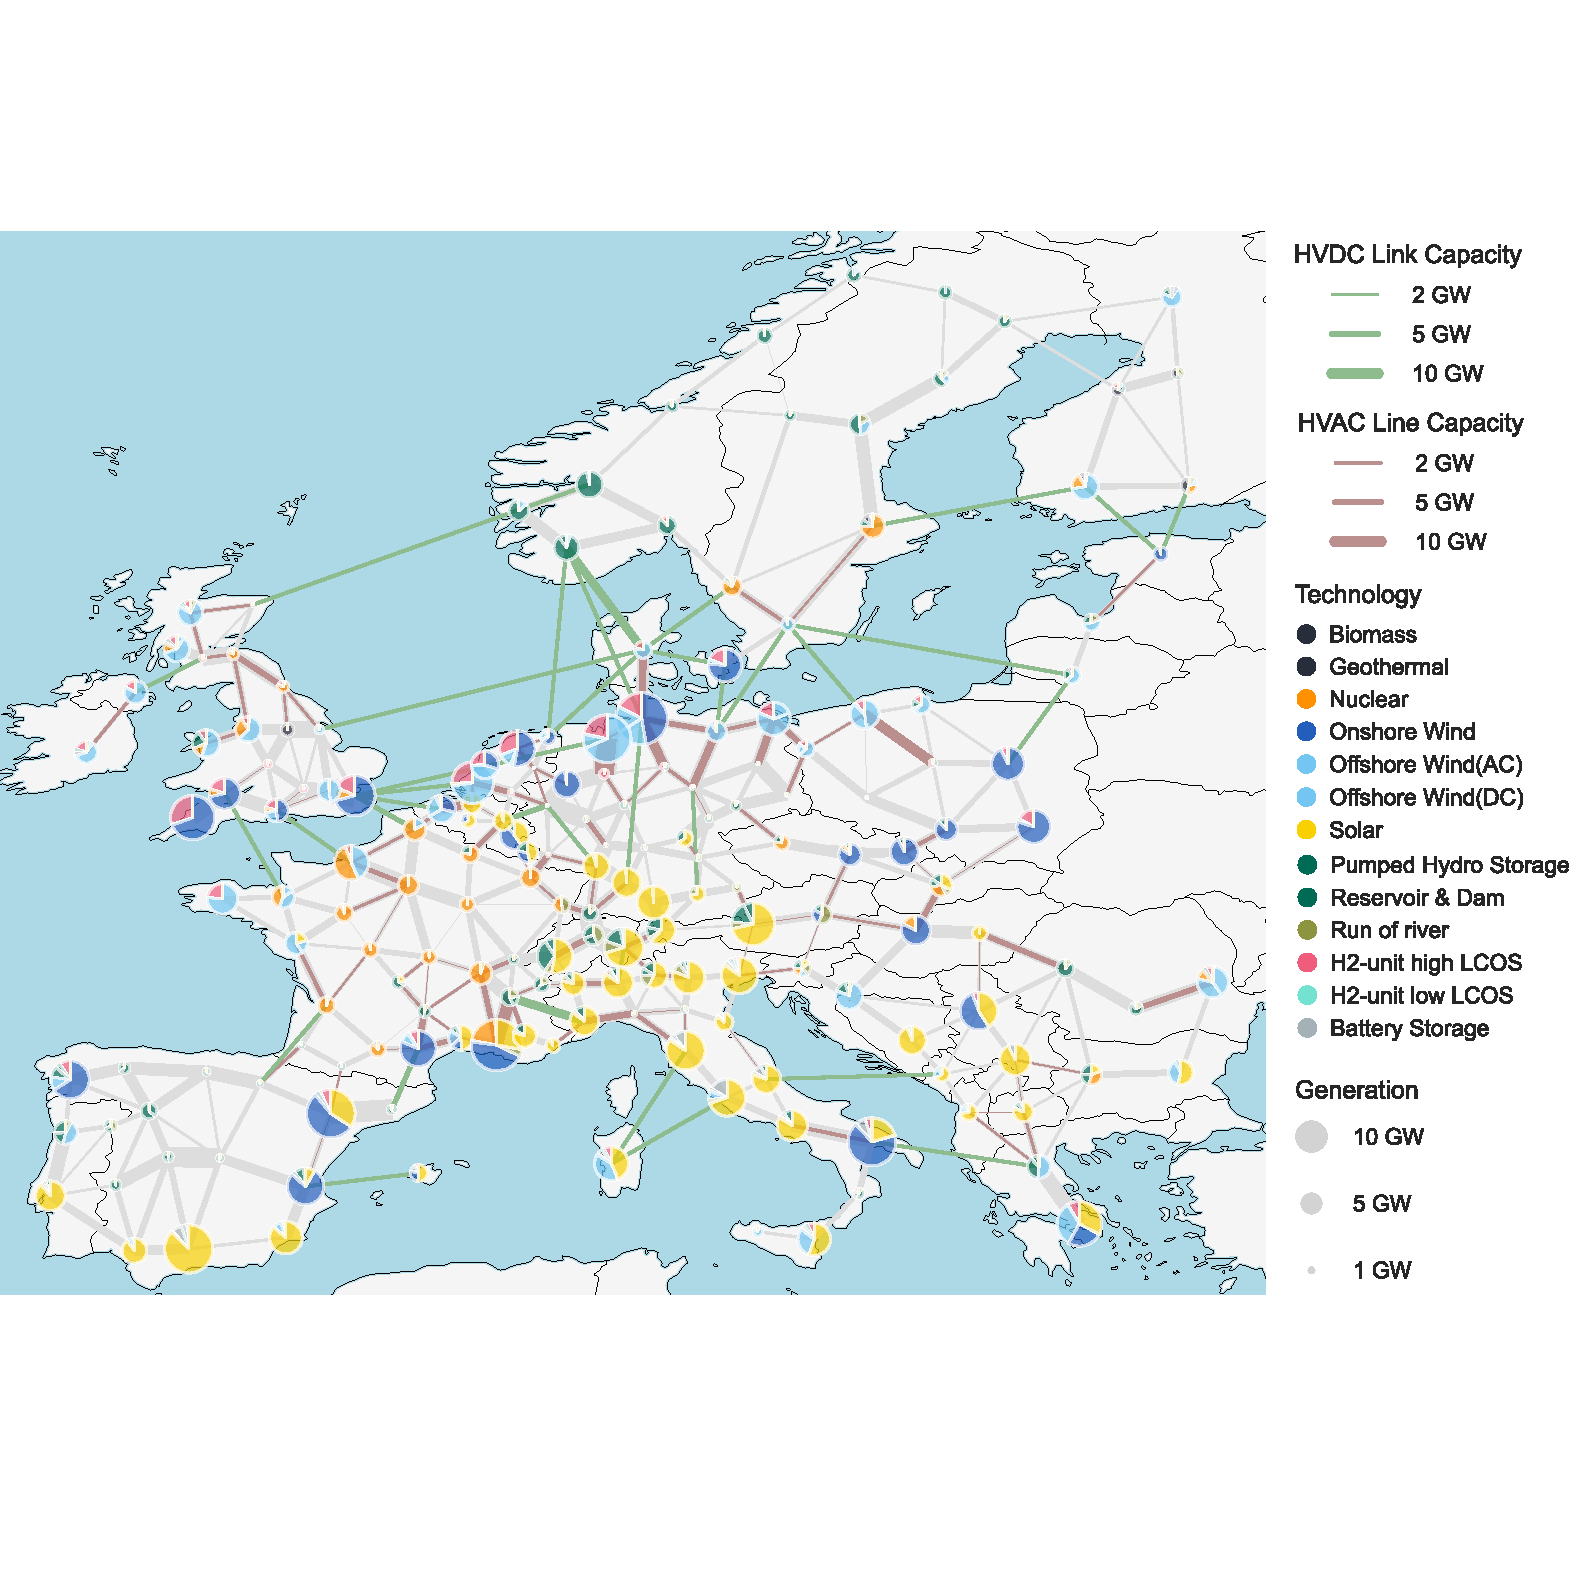
\includegraphics[width = 0.5\textwidth]{Figures/EU-generation-map2.pdf}}
% \caption{Map of planned and existing transmission lines in Africa.}
% \label{EU-Map}
% \end{figure}

%%%% VERSION TWO
\begin{figure}[htbp]
\centerline{\includegraphics[trim={0cm 0.1cm 0cm 3cm},clip,width = 0.5\textwidth]{Figures/EU-generation-map.pdf}}
\caption{PyPSA-Eur outputs to envision planned achievements in the future African model. Map showing optimal generation, storage and network expansion in Europe under a 100\% emission reduction scenario and technology data for 2030. Light grey lines showing the existing installed network capacity~\cite{parzen-neumann-ea-2021}.}
\label{EU-Map}
\end{figure}

%%%% Africa plot with transmission lines & substations [MATIN]

\begin{figure}[htbp]
\centerline{\includegraphics[trim={4cm 8cm 4cm 8cm},clip,width = 0.5\textwidth]{Figures/africa_transmission_network_and_substations.png}}
\caption{The map suggest that a large amount of transmission line and substation data is available in Africa. However, the data should be extended and validated as far as possible which can be accomplished in future endeavours. Blue lines show planned and existing transmission lines over 110 kV in Africa and the MENA region. Orange marked points show existing substations on transmission level. Data is available at https://energydata.info/dataset/africa-electricity-transmission-and-distribution-grid-map-2017 \& OpenStreetMap}.
\label{AfricaMApTransmission}
\end{figure}

The model being developed by PyPSA meets Africa will build on the successes of PyPSA-Eur.
It will be the first model of the African transmission grid at a high, adjustable spatial resolution.
Moreover, this is done with a modular workflow based on open data meeting the FAIR principles~\cite{wilkinson-dumontier-ea-2016}.
As a result, the model can easily be updated with improved data as it becomes available.

The project aims to work as much as possible with existing open source libraries and working code bases; see also the later subsections.
This will allow us to couple the African model with PyPSA-Eur, enabling cross-beneficial source code development, intercontinental studies, and a larger user base.
Additionally, we foresee to add the sector-coupling of PyPSA-Eur-Sec to the African model.
The ultimate goal is to create a long-term maintained and supported OS model that is useful for industry, research and policy purposes.


% further accelerate the integration of different RES technologies such as solar, wind, tidal and other marine sources and additionally smart grid objects such as batteries and electric vehicles. As shown in \cref{AfricaMApTransmission}, as an initial step to map the existing transmission lines.  This study uses the dataset made available by Onsset which ``includes planned and existing grid lines for all continental African countries and Madagascar, as well as the Middle East region. The lines range in voltage from sub-kV to 700 kV EHV lines.'' It should be noted that there is a large variation in availability of data for different countries.


The project is split into multiple work packages which are layed out in the next subsections including an outlook on the methodology planned for each work package:

\begin{enumerate}
    \item Demand modelling
    \item Conventional generator modelling
    \item RES modelling
    \item Land coverage constraint modelling
    \item Network and substation modelling
    \item Data creation and validation 
\end{enumerate}

We aim to complete a working prototype of our model by end of 2021.

\subsection{Demand modelling} %%% Johannes. Desen reviewed
In order to model the electricity consumption, GlobalEnergyGIS (GEGIS) will be employed to obtain a hourly time-series of demand.
GEGIS applies a machine learning (ML) approach based on existing electricity demand time-series data, population densities and spatially resolved income data.
This data is complemented with scenario information from the Shared Socioeconomic Pathways (SSP) and weather data from ERA5 to generate hourly outputs for arbitrary regions until 2050.

% \todo[inline]{I haven't checked the following sentence and can neither confirm nor deny its correctness.}
% GEGIS follows the open GIS standards of the Open Geospatial Consortium and is operated as shown in \cref{GEGIS}.

% \begin{figure}[htbp]
% \centerline{\includegraphics[width = 0.45\textwidth]{Figures/GeGIS.png}}
% \caption{A screenshot from GEGIS [REF!].}
% \todo[inline]{Where is this figure from? I have never seen a GUI for GEGIS.}
% \label{GEGIS}
% \end{figure}

\subsection{Conventional generator modelling} %%% Koen. Desen reviewed
Regarding the modelling of conventional generators, data is made available through the Global Power Plant Database (GPPD)~\cite{globalenergyobservatory-google-ea-2018}, which is one of the principle open global power plant databases.
Commercial power plant databases with restricted access historically was dominant in policy-making and research, but in recent years open databases are closing the gap.
For conventional generation (i.e. coal, natural gas, oil, hydro), the GPPD has a coverage of 80--100\% (depending on the category) in terms of installed capacity, when compared to the state-of-the-art commercial sources~\cite{byers-friedrich-ea-2019}.

The database can be integrated with PyPSA using the \emph{powerplantmatching} tool~\cite{gotzens-heinrichs-ea-2019}.
Additionally, it also enables integration with other databases.
As such, our model can incorporate new and improved datasets as they become available.

Hydro power plays an important role in Africa, and is expected to continue doing so.
While the GPPD includes data on existing hydro plants, we can also use existing geospatial analyses~\cite{korkovelos-mentis-ea-2018} of the potential for new hydro plants.


\subsection{RES generator modelling} %%% Johannes. Desen reviewed
In terms of RES modelling, the project aims to model both the existing and planned generators. As widely known, weather data such as wind speed/direction and solar irradiation play an important role in RES modelling. Using \emph{Atlite}\footnote{\url{https://github.com/PyPSA/atlite}} package, spatially resolved potentials and hourly time-series of wind, solar and ocean data are modelled into generation output from different plants. 

Currently, \emph{atlite} supports wind turbines and solar PV as generators and uses ERA5 (i.e. hourly estimates of atmospheric and oceanic climate variables) complemented with irradiation data from SARAH2.
% \todo[inline]{Desen: I think we need a ref for ERA5 and SARAH2 so that the reader can access this info. This can be the Atlite docs - https://atlite.readthedocs.io/en/latest/}
The project aims to increase the variety of RES models to include CSP and marine energy like wave or tidal generators.

% RES will likely be the cornerstone of most future energy systems.
% For this project, spatially resolved potentials and hourly resolved time-series for energy generation from wind, solar and ocean sources will be modelled using established and updated methodologies with the Python package \emph{atlite}\footnote{\url{https://github.com/PyPSA/atlite}}.
%TODO: add a reference for atlite. See https://github.com/openjournals/joss-reviews/issues/3204 for the issue at JOSS.
% Unfortunately, it looks the paper is not going to go into preprint before our submission deadline. The URL should do for now, and hopefully we can cite it in the final version of this paper.

\subsection{Land coverage constraint modelling} %% Desen
Different types of land use, extreme terrain conditions and protected areas constrain the eligible areas for RES development, placement of transmission lines, etc. Both land and sea/ocean constraints can be integrated in \emph{atlite}. In addition to the oceanic climate factors, water depth is a constraint for offshore and marine energy turbines where bathymetric dataset will be obtained from General Bathymetric Chart of the Oceans (GEBCO). Protected areas such as national parks will be researched and integrated into the model which provides an aspect of novelty. Population distribution and land cover surveys such as Corine Land Cover can be used to indicate regions with high population densities, farm land, extreme terrain, etc.

% \todo[inline]{Desen: needs reference for GEBCO, etc.}


% \begin{itemize}
% % \item water depth we can include/exclude based on the GEBCO bathymetric dataset. Also used in PyPSA-EUR
% % 	land usage/coverage/protected areas (tool): 
% % \item Can be exlucded using atlite. Severin Rydberg created GLAES for this purpose a few years ago but that tool is no longer maintained so Fabian Hofmann from the atlite team included that functionality into atlite recently.
	
% % \item land usage/coverage/protected areas (data): This is were it becomes tricky.
% \item  Maybe global corine is suitable for land usage. Protected areas would still need to be included somehow. Potentially also population density (were again I know datasets exist but I do not know how applicable they are)
% \end{itemize}


% Ok, here are just my thoughts, can someone else assist with selection/formulation?
% * I don't know which data set we can use for Land coverage and protected areas
% * Data sets I know of are limited to Europe, NA, Asia
% * Maybe the Corine dataset is available for Africa/ww and would provide land usage data 
% * In addition we would need a data set for protected areas. I have no idea what do use here
% * Niclas Mattsson used with GEGIS also some datasets and he managed world-wide coverage. Maybe we find our answer there already?
% * Yes, modelling with Atlite should be possible

\subsection{Network and substation modelling} %%% Max and Matin. Not yet reviewed
The network topology for Africa will mainly be extracted from a dataset compiled by the World Bank Group~\cite{arderne-2017}, which is based on a number of different sources. The dataset includes 1818 inputs for transmission lines (above 110 kV), the total length is 4204 km. Similar to PyPSA-Eur\cite{PyPSAEur}, the mapped data will be enriched by typical physical parameters such as length dependent resistance and reactance, current thermal level and apparent power limit.

The substation geolocation with voltage level will be extracted from Open Street Maps (OSM). To be computable on typical 16GB RAM computers, a relatively new efficient OSM extraction package `esy-osmfilter'~\cite{pluta-lunsdorf-2020} will be applied that is four times faster than the common alternative, OSMOSIS~\cite{henderson-2020}. Initial results from the OSM extraction process (see result in \cref{AfricaMApTransmission}) show 2721 transmission substation data points for Africa.

As for PyPSA-Eur, the country shapes and bus location will be used to split areas into Voronoi cells which are assumed to be connected to low voltage networks. Each of the Voronoi cell contains information on existing power plant capacities, renewable resource potential timeseries, as well as demand timeseries at the substation location. The spatial model resolution can be changed by aggregating the cells by k-means clustering.

\subsection{Data creation and validation} % Max and Matin. Desen reviewed.

The amount of data on energy assets might vary per country (see \cref{AfricaMApTransmission}). The missing data can be either added by local energy authorities or using asset recognition techniques on satellite imagery. It is known that data from centralised organisation such as the European Network of Transmission System Operator (ENTSO-E) may be out-of-date or unreliable \cite{gotzens-heinrichs-ea-2019,PyPSAEur}. Therefore, ML techniques can be applied to both validate existing data and create new data from satellite images.

In the concept of electricity grid, ML can be used to create missing data and increase manual validation speed by at least 33-fold compared to  manual mapping strategies~\cite{developmentseed-2018}. 
% ML approaches should not be seen in near future to replace a human validation step as the accuracy is not satisfactory. However, ML approaches are an ideal complement to current mapping techniques and can speed up the human validation process, for instance, by providing only images that are highly likely to contain the specific energy asset. 
Using ML techniques, high voltage lines, substations~\cite{developmentseed-2018}, solar PV \cite{dehoog-maetschke-ea-2020} and wind turbines~\cite{zhou-irvin-ea-2019} were identified from satellite imagery. This involves creating a training data set which consists of marking energy assets on the images. Once the algorithm is trained, it is able identify the chosen energy asset in several other images. The information gained from ML can be, for instance, area and inclination of PV arrays that may be used to estimate their annual energy output. Other physical parameters such as voltage level of substations and age of assets might be also possible to extract by training ML on specific substation data and analysing satellite images over multiple years.

The 'PyPSA meets Africa' project prioritises the creation of validated substation and high voltage line datasets which will be made publicly available in line with the OS approach. There are plans to use ML for identification of other energy assets in the future.

\section{Conclusions}
In this paper, we discussed the importance of OS energy systems modelling in the African continent. The existing work in terms of both academic literature, technical reports (e.g. by United Nations) and grass roots initiatives were reviewed. Lastly, we also presented our proposed roadmap to open energy modelling and data sharing in Africa which is aimed to have a wider audience with further integrated technologies such as marine energy and grid-scale batteries scheduled to increase the resiliency of the African grid \cite{}. This is expected to accelerate the simulation and hence, later integration of renewable energy technologies.

\section*{Acknowledgments}
EPRSC Doctoral Training Partnership (EP/R513209/1) and the EPSRC Centre for Energy System Integration (EP/P001173/1) are acknowledged for their support.
All funding bodies and everyone who helped improve the paper but did not contribute to the writing/analysis/etc.


% \printbibliography

\bibliographystyle{IEEEtran}
% \todo[inline]{Desen: Papers  that  have  not  been  published,even  if  they  have  been  submitted  for  publication,  should  be cited as “unpublished” [4]. Papers that have been accepted for publication should be cited as “in press” [5]}
\bibliography{bibliography}

\end{document}


% \begin{thebibliography}{00}
% \bibitem{b1} G. Eason, B. Noble, and I. N. Sneddon, ``On certain integrals of Lipschitz-Hankel type involving products of Bessel functions,'' Phil. Trans. Roy. Soc. London, vol. A247, pp. 529--551, April 1955.
% \bibitem{b2} J. Clerk Maxwell, A Treatise on Electricity and Magnetism, 3rd ed., vol. 2. Oxford: Clarendon, 1892, pp.68--73.
% \bibitem{b3} I. S. Jacobs and C. P. Bean, ``Fine particles, thin films and exchange anisotropy,'' in Magnetism, vol. III, G. T. Rado and H. Suhl, Eds. New York: Academic, 1963, pp. 271--350.
% \bibitem{b4} K. Elissa, ``Title of paper if known,'' unpublished.
% \bibitem{b5} R. Nicole, ``Title of paper with only first word capitalized,'' J. Name Stand. Abbrev., in press.
% \bibitem{b6} Y. Yorozu, M. Hirano, K. Oka, and Y. Tagawa, ``Electron spectroscopy studies on magneto-optical media and plastic substrate interface,'' IEEE Transl. J. Magn. Japan, vol. 2, pp. 740--741, August 1987 [Digests 9th Annual Conf. Magnetics Japan, p. 301, 1982].
% \bibitem{b7} M. Young, The Technical Writer's Handbook. Mill Valley, CA: University Science, 1989.
% \end{thebibliography}

% \section{Prepare Your Paper Before Styling}
% Before you begin to format your paper, first write and save the content as a 
% separate text file. Complete all content and organizational editing before 
% formatting. Please note sections \ref{AA}--\ref{SCM} below for more information on 
% proofreading, spelling and grammar.

% Keep your text and graphic files separate until after the text has been 
% formatted and styled. Do not number text heads---{\LaTeX} will do that 
% for you.

% \subsection{Abbreviations and Acronyms}\label{AA}
% Define abbreviations and acronyms the first time they are used in the text, 
% even after they have been defined in the abstract. Abbreviations such as 
% IEEE, SI, MKS, CGS, ac, dc, and rms do not have to be defined. Do not use 
% abbreviations in the title or heads unless they are unavoidable.

% \subsection{Units}
% \begin{itemize}
% \item Use either SI (MKS) or CGS as primary units. (SI units are encouraged.) English units may be used as secondary units (in parentheses). An exception would be the use of English units as identifiers in trade, such as ``3.5-inch disk drive''.
% \item Avoid combining SI and CGS units, such as current in amperes and magnetic field in oersteds. This often leads to confusion because equations do not balance dimensionally. If you must use mixed units, clearly state the units for each quantity that you use in an equation.
% \item Do not mix complete spellings and abbreviations of units: ``Wb/m\textsuperscript{2}'' or ``webers per square meter'', not ``webers/m\textsuperscript{2}''. Spell out units when they appear in text: ``. . . a few henries'', not ``. . . a few H''.
% \item Use a zero before decimal points: ``0.25'', not ``.25''. Use ``cm\textsuperscript{3}'', not ``cc''.)
% \end{itemize}

% \subsection{Equations}
% Number equations consecutively. To make your 
% equations more compact, you may use the solidus (~/~), the exp function, or 
% appropriate exponents. Italicize Roman symbols for quantities and variables, 
% but not Greek symbols. Use a long dash rather than a hyphen for a minus 
% sign. Punctuate equations with commas or periods when they are part of a 
% sentence, as in:
% \begin{equation}
% a+b=\gamma\label{eq}
% \end{equation}

% Be sure that the 
% symbols in your equation have been defined before or immediately following 
% the equation. Use ``\eqref{eq}'', not ``Eq.~\eqref{eq}'' or ``equation \eqref{eq}'', except at 
% the beginning of a sentence: ``Equation \eqref{eq} is . . .''

% \subsection{\LaTeX-Specific Advice}

% Please use ``soft'' (e.g., \verb|\eqref{Eq}|) cross references instead
% of ``hard'' references (e.g., \verb|(1)|). That will make it possible
% to combine sections, add equations, or change the order of figures or
% citations without having to go through the file line by line.

% Please don't use the \verb|{eqnarray}| equation environment. Use
% \verb|{align}| or \verb|{IEEEeqnarray}| instead. The \verb|{eqnarray}|
% environment leaves unsightly spaces around relation symbols.

% Please note that the \verb|{subequations}| environment in {\LaTeX}
% will increment the main equation counter even when there are no
% equation numbers displayed. If you forget that, you might write an
% article in which the equation numbers skip from (17) to (20), causing
% the copy editors to wonder if you've discovered a new method of
% counting.

% {\BibTeX} does not work by magic. It doesn't get the bibliographic
% data from thin air but from .bib files. If you use {\BibTeX} to produce a
% bibliography you must send the .bib files. 

% {\LaTeX} can't read your mind. If you assign the same label to a
% subsubsection and a table, you might find that Table I has been cross
% referenced as Table IV-B3. 

% {\LaTeX} does not have precognitive abilities. If you put a
% \verb|\label| command before the command that updates the counter it's
% supposed to be using, the label will pick up the last counter to be
% cross referenced instead. In particular, a \verb|\label| command
% should not go before the caption of a figure or a table.

% Do not use \verb|\nonumber| inside the \verb|{array}| environment. It
% will not stop equation numbers inside \verb|{array}| (there won't be
% any anyway) and it might stop a wanted equation number in the
% surrounding equation.

% \subsection{Some Common Mistakes}\label{SCM}
% \begin{itemize}
% \item The word ``data'' is plural, not singular.
% \item The subscript for the permeability of vacuum $\mu_{0}$, and other common scientific constants, is zero with subscript formatting, not a lowercase letter ``o''.
% \item In American English, commas, semicolons, periods, question and exclamation marks are located within quotation marks only when a complete thought or name is cited, such as a title or full quotation. When quotation marks are used, instead of a bold or italic typeface, to highlight a word or phrase, punctuation should appear outside of the quotation marks. A parenthetical phrase or statement at the end of a sentence is punctuated outside of the closing parenthesis (like this). (A parenthetical sentence is punctuated within the parentheses.)
% \item A graph within a graph is an ``inset'', not an ``insert''. The word alternatively is preferred to the word ``alternately'' (unless you really mean something that alternates).
% \item Do not use the word ``essentially'' to mean ``approximately'' or ``effectively''.
% \item In your paper title, if the words ``that uses'' can accurately replace the word ``using'', capitalize the ``u''; if not, keep using lower-cased.
% \item Be aware of the different meanings of the homophones ``affect'' and ``effect'', ``complement'' and ``compliment'', ``discreet'' and ``discrete'', ``principal'' and ``principle''.
% \item Do not confuse ``imply'' and ``infer''.
% \item The prefix ``non'' is not a word; it should be joined to the word it modifies, usually without a hyphen.
% \item There is no period after the ``et'' in the Latin abbreviation ``et al.''.
% \item The abbreviation ``i.e.'' means ``that is'', and the abbreviation ``e.g.'' means ``for example''.
% \end{itemize}
% An excellent style manual for science writers is \cite{b7}.

% \subsection{Authors and Affiliations}
% \textbf{The class file is designed for, but not limited to, six authors.} A 
% minimum of one author is required for all conference articles. Author names 
% should be listed starting from left to right and then moving down to the 
% next line. This is the author sequence that will be used in future citations 
% and by indexing services. Names should not be listed in columns nor group by 
% affiliation. Please keep your affiliations as succinct as possible (for 
% example, do not differentiate among departments of the same organization).

% \subsection{Identify the Headings}
% Headings, or heads, are organizational devices that guide the reader through 
% your paper. There are two types: component heads and text heads.

% Component heads identify the different components of your paper and are not 
% topically subordinate to each other. Examples include Acknowledgments and 
% References and, for these, the correct style to use is ``Heading 5''. Use 
% ``figure caption'' for your Figure captions, and ``table head'' for your 
% table title. Run-in heads, such as ``Abstract'', will require you to apply a 
% style (in this case, italic) in addition to the style provided by the drop 
% down menu to differentiate the head from the text.

% Text heads organize the topics on a relational, hierarchical basis. For 
% example, the paper title is the primary text head because all subsequent 
% material relates and elaborates on this one topic. If there are two or more 
% sub-topics, the next level head (uppercase Roman numerals) should be used 
% and, conversely, if there are not at least two sub-topics, then no subheads 
% should be introduced.

% \subsection{Figures and Tables}
% \paragraph{Positioning Figures and Tables} Place figures and tables at the top and 
% bottom of columns. Avoid placing them in the middle of columns. Large 
% figures and tables may span across both columns. Figure captions should be 
% below the figures; table heads should appear above the tables. Insert 
% figures and tables after they are cited in the text. Use the abbreviation 
% ``Fig.~\ref{fig}'', even at the beginning of a sentence.

% \begin{table}[htbp]
% \caption{Table Type Styles}
% \begin{center}
% \begin{tabular}{|c|c|c|c|}
% \hline
% \textbf{Table}&\multicolumn{3}{|c|}{\textbf{Table Column Head}} \\
% \cline{2-4} 
% \textbf{Head} & \textbf{\textit{Table column subhead}}& \textbf{\textit{Subhead}}& \textbf{\textit{Subhead}} \\
% \hline
% copy& More table copy$^{\mathrm{a}}$& &  \\
% \hline
% \multicolumn{4}{l}{$^{\mathrm{a}}$Sample of a Table footnote.}
% \end{tabular}
% \label{tab1}
% \end{center}
% \end{table}

% \begin{figure}[htbp]
% \centerline{\includegraphics{fig1.png}}
% \caption{Example of a figure caption.}
% \label{fig}
% \end{figure}

% Figure Labels: Use 8 point Times New Roman for Figure labels. Use words 
% rather than symbols or abbreviations when writing Figure axis labels to 
% avoid confusing the reader. As an example, write the quantity 
% ``Magnetization'', or ``Magnetization, M'', not just ``M''. If including 
% units in the label, present them within parentheses. Do not label axes only 
% with units. In the example, write ``Magnetization (A/m)'' or ``Magnetization 
% \{A[m(1)]\}'', not just ``A/m''. Do not label axes with a ratio of 
% quantities and units. For example, write ``Temperature (K)'', not 
% ``Temperature/K''.